\chapter{Results}

Having detailed both the method used for recommendation and the actual implementation of that method, the discussion now moves to the method for evaluating the results and the presentation of the results themselves in order to demonstrate the efficacy of the method.

First the method of evaluating the results is described; for such a large dataset this is a challenging question, and it is not yet well-defined for this research area. The selection of the distinguished users is then described and their effect on the evaluation methods is considered before arriving at several metrics for evaluating the results.

Next the baseline results are shown using the established metrics. Finally, variations on the algorithm are experimented with and their results presented in order to establish which parameters and edge types are the most valuable for this task and whether the algorithm can be improved over its baseline result.


\section{Evaluation Methodology}

\subsection{Challenges}

A review of the existing research on content recommendation discussed in Section~\ref{sec:ContentRecommendationResearch}, reveals no consensus on how best to evaluate the results of a recommendation method. This is due primarily to two separate but related issues: the lack of a common dataset and the lack of ground truth judgements on the relevance of either content or users.

None of the research projects on Twitter content recommendation reviewed in Section~\ref{sec:ContentRecommendationResearch} used the same set of Twitter data for their experiments. All of the researchers used the Twitter API to download their own datasets of varying sizes and using various procedures. Because of this the datasets turn out to be very different in terms of size, user composition, and tweet content, which makes results difficult to compare between papers. The creation of the microblog track of the Text Retrieval Conference (TREC) was accompanied by a very large collection of tweet data which may be commonly used in the future, but as discussed in Section~\ref{sec:SelectingADataset}, it was not sufficient for this project.

The bigger issue, however, is the lack of a set of ground truth judgements of the relevance of tweets and users in any dataset. One obvious cause of this is the lack of a canonical dataset upon which recommendations are made. Perhaps if ground truth judgements were available such a dataset would come into common usage, but the fact is that the job is too complex to realistically be performed reliably for any decent sample size. The content and users that are relevant for one user would be vastly different from the content and users relevant for another. And any database of a usable size would have millions and millions of tweets and users, far too many for all of them to be judged for even one user.


\subsection{Distinguished User Selection}

With these challenges in mind, it was necessary to develop methods of evaluating the performance of the algorithm that did not rely on a pre-judged set of relevant content and users. The first step was to choose distinguished users to whom the content should be recommended. For privacy reasons, those users are not named here. Overall, three users were chosen.

Two users were chosen because they are known personally by the author and are long-time users who are present in the dataset. These facts made them ideal candidates for the user studies discussed in Section~\ref{sec:UserStudy}. Both of these users are computer scientists, so technology is a major interest, but there are some distinguishing interests as well. These two users will be known as users $K_{i}$ and $K_{j}$, with the choice of K meant to indicate that they are the users {\bf K}nown to the author. Both users joined Twitter in early 2009. In addition to their common interests, user $K_{i}$ was also interested in languages, amongst other subjects, while one of user $K_{j}$'s top interests was mobile phone applications.

The other user was chosen because his interests are clear and easy to distinguish and because he was well connected to the small sample of tweets that were used during initial implementation. This user has more than 7,000 followers as of this writing, up from approximately 3,700 three years ago when the dataset was collected. As of this writing he has published nearly 25,000 tweets. His interests are also in technology, but with a business focus. A large number of his current followees are technology entrepreneurs, but he also posts tweets and has followees related to popular culture such as films, television, and music. This user will be known as user $U$, indicating that he is {\bf U}nknown to the author.



\subsection{User Study}
\label{sec:UserStudy}

The goal of the user study is primarily to determine whether the content recommended to the users was of interest to the distinguished user.

A user study is perhaps the closest method of evaluation to a set of ground truth relevance judgements, though on a smaller scale. For the tweets ranked by the users it is possible to say with certainty how relevant they are and thus to evaluate the precision of the algorithm. The user study could obviously only be performed on the users known to the author, which was part of what motivated the choice of known users as distinguished users.

One major drawback of the user study is that it recommends content to these users based on what was happening three years ago. Thus, the recommendations are based on the interests of three years ago which may no longer be relevant. Before filling out the user survey these users were asked to put themselves in the frame of reference of what might have been interesting to them three years ago, but this is obviously inexact, so the efficacy of user study depends largely on the idea that interests change slowly.

The user studies consisted of two components: recommending users and recommending individual tweets. 

For recommending individual tweets, the top thirty tweets from each experiment that was run, retrieved as described in Section~\ref{sec:RetrievingResults}, were retrieved after the algorithm was run. Crucially, tweets which were an @reply to another user were filtered out since a user would not see those if they were to follow the user in question. After running this procedure for all of the experiments, there were approximately 150 tweets for each user to rank.

These filtered tweets were then presented to the user in a random order and each user was asked to rank each of the tweets on a scale from 1 to 5 using the values from Table~\ref{tab:UserRankingScoresForTweets}. From these scores, the precision was evaluated by considering tweets scored as either 4 or 5 to be relevant tweets and seeing how many of the top 20 tweets were relevant. Recall is not really possible to evaluate with a currently existing Twitter dataset, unfortunately, because of the lack of ground truth relevance judgements on the Twitter data.


\begin{table}
\centering
\begin{tabular}{c|l}
{\bf Score} & {\bf Description of tweets with this score} \\ \hline
1 & Not relevant at all, e.g. non-English tweets \\ \hline
2 & Useless tweets \\ \hline
3 & Average tweet; not particularly useful, but not completely without value \\ \hline
4 & Relevant or interesting tweet \\ \hline
5 & Very relevant tweets \\
\end{tabular}
\caption{User ranking scores for tweets}
\label{tab:UserRankingScoresForTweets}
\end{table}


Recommending users proceeded in a largely similar manner. A surprising number of the recommended users either no longer appear as users or have set their Twitter feeds to be private, preventing effective evaluation, so the option for the users to rate the user as ``not available'' was added. These users were then filtered out of the results when calculating precision.

For each recommended user, the distinguished user under study was presented with a link to their Twitter page so that their profile and recent tweets could be viewed. Each user to be ranked was presented in random order. The users under study were then asked to rank the recommended users according the scale of Table~\ref{tab:UserRankingScoresForUsers}, which is largely similar to the scale for ranking tweets. The results of this ranking were then used in the same way to determine precision scores by considering users scored as either 4 or 5 to be relevant users.

As with the tweets, it was not really possible to evaluate the recall of current users because it is not possible to say how many total relevant users there are.


\begin{table}
\centering
\begin{tabular}{c|l}
{\bf Score} & {\bf Description of users with this score} \\ \hline
0 & Users whose Twitter feeds are no longer available \\ \hline
1 & Not relevant at all, e.g. users tweeting in another language \\ \hline
2 & Uninteresting users \\ \hline
3 & Average user; not particularly interesting, but not without value \\ \hline
4 & Interesting users;  includes users who once were followed but no longer are \\ \hline
5 & Users that the distinguished user now follows \\
\end{tabular}
\caption{User ranking scores for users}
\label{tab:UserRankingScoresForUsers}
\end{table}


\subsection{Comparison to Current Tweets}
\label{sec:ComparisonToCurrentTweets}

The user study is effective for evaluating the results for the known users but is subject to biases and changes in interests and does nothing for evaluating the results for unknown or unavailable users. As such, it was also necessary to develop more automated techniques.

Perhaps the best possibility would be to use the closest thing to a ground truth dataset that exists: the list of all the tweets that a particular distinguished user retweeted. If the user's own connections to each of these tweets were severed then it would be possible to test just how many of these tweets were actually recommended. This presents two major problems, however. First, because the dataset is limited to only approximately 20\%-30\% of the tweets that were published in the time period, many of the initial tweets were missed and only their retweets were captured. Second, in the small time period being examined, most distinguished users would be unlikely to retweet even one or two tweets, leaving insufficient data for evaluation.

A more realistic technique is to assume that a user's interests remain static between the time period represented by the dataset and the present day. This makes it possible to compare the tweets recommended by the system to the tweets that the user is actually interested in while using a separate data source to avoid overfitting.

As described by \cite{Welch2011} and mentioned elsewhere in this dissertation, retweets are the most effective means of determining which content a person is interested in. Thus, each tweet recommended by the system can be compared to each of the most recent retweets from the present day twitter stream of the user for whom the recommendations are being created, and the score can be averaged together. These numbers can be compared to a baseline created by comparing each tweet in the system to the reference tweets and taking an average of their similarity scores. This process can be repeated for tweets that the distinguished user has authored.

For this project, the method of determining similarity was the modified cosine similarity metric as described in Section~\ref{sec:TweetScoresImplementation}. Because of the large number of tweets in the database the baseline against which these numbers were compared was determined by taking the average of the similarity scores for 2,500 tweets rather than for the entire collection. Looking at the similarity scores for after each batch of 500 tweets was incorporated into the average showed that the average scores did not change very much from the score after evaluating the first 500, validating the choice of 2,500 as the limit.

As with all of the means of evaluation, this is an imperfect measurement. Given their technical interests and the fast-paced nature of that field, many of the technologies that these users are interested in today may not have existed at the time the data was collected. Still, it does allow a comparison to show that the recommendations provided have value above random recommendation and because it is automated it allows far more documents to be ranked than the user study.



\subsection{Comparison to Current Network State}
\label{sec:ComparisonToCurrentNetwork}

Much of the research on link prediction in social networks focuses on predicting whether links will be created between users in the future, and the evaluation involves comparing the predicted links to those actually formed later. For this project, the only data available on the state of the social graph is that of the dataset and that of the present day.

Thus, one evaluation method used was to compare the users recommended for each distinguished user to the set of actual followees of that person in the present social network. For the two known users it was also possible to include users who were included in the recommendations whom the distinguished user may once have followed but no longer does. The number of recommended users likely to be in the set of present-day followees is extremely small given that most users follow a small set of people, but by comparing the number of users in the top 20 recommended users who overlap with the present-day followee list to the probability of a random user appearing in that list it is possible to demonstrate that the recommendations have value.

Calculating the probability of a random user from the data being amongst the present-day followees requires a major assumption: that the network today is the same size and has the same users as the network of the dataset. This is necessary because there simply is not data available for the relevant network information at any point except the dataset used here and the present day. This assumption is obviously not true, but it means that the actual probability is smaller than the calculated probability, so the calculated probability can be taken as an upper bound. Using this assumption, it is possible to calculate the approximate probability that a random user would be a present-day followee of the distinguished user with the following formula:


\begin{center}
\[
\frac{\Delta_{followees} }{count(user\ vertices) - count(dataset\ followees)}
\]
\end{center}


User $K_{i}$ has 43 followees in the dataset used here compared to 443 today and 72 followers in the dataset used here compared to 791 today. In the set of tweets studied here, this user authored 2 tweets, one of which was a retweet. He also had more than 6,000 edges emanating from his user vertex. Most of these edges were content edges since one of this user's tweets mentioned a very popular hashtag on this particular day.

User $K_{j}$ has 105 followees in the dataset compared to 505 today and 87 followers in the dataset used here compared to 495 today. He also had 2 tweets, one of them a retweet and one of them an at-reply. He was connected to tweets by a mere 57 edges.

User $U$ has 279 followees in the dataset compared to 442 today to go along with 3,720 followers in the dataset compared to 7,191 today. Given these numbers, the probability that a random user would be a present day followee of each user is listed in Table~\ref{tab:RandomUserFolloweeProb}. These probabilities can then be compared to the number of users recommended by the algorithm who the user currently follows in order to establish the value of the algorithm.

\begin{table}
\centering
\begin{tabular}{c|c|l}
{\bf User} & {\bf $\Delta_{followees}$ } & {\bf Probability} \\ \hline
$U$ & 163 &  0.04\%   \\ \hline
$K_{i}$ & 400 & 0.10\% \\ \hline
$K_{j}$ & 400 & 0.09\% \\
\end{tabular}
\caption{Probability of a random user being added as a followee}
\label{tab:RandomUserFolloweeProb}
\end{table}


\section{Results}

This section describes the results which were obtained. Most of the scores are presented in the form of precision at rank and are based on the results of the user study. These scores are labelled in the various tables as `P@5', `P@10', `P@15', and `P@20', representing the precision at 5, 10, 15, and 20. Recall from above that for purposes of calculating precision, a tweet or user is considered to be relevant if it was rated at either 4 or 5 in the user study. Since user $U$ was not part of the user study, he has no numbers for this measurement. All of the rankings for the known users $K_{i}$ and $K_{j}$ also include a result for the average score at rank 5, 10, 15, and 20, which imparts some additional information about the quality of the rankings.

For the user recommendation results, the tables also include a column for `\% 5s @ 5', `\% 5s @ 10', etc. This value is the percentage of users rated as a 5 at various ranks in the recommendations. This corresponds to the users that they actually have started following since this data was collected in 2009, though in the case of the users included in the user study, at least one or two of the users ranked as 5 were users who they did not follow before seeing the recommendation. This measurement is the metric described in Section~\ref{sec:ComparisonToCurrentNetwork} of comparing the list of recommended users to the users that the distinguished user now follows. Because it is possible to determine this for all users, this number is included for user $U$. These numbers compare very favourably with the chance of a random user appearing in this list as discussed in Section~\ref{sec:ComparisonToCurrentNetwork}, demonstrating that the user recommendations are very useful, though as will become apparent most of the value in user recommendations comes from the initial score.

For most of the variations on the baseline results only one user was studied for each variation, providing a very small sample size. So while the results are very promising for many of the experiments, caution is warranted because there simply is not very much information. The need for improving the sample size is discussed further in Chapter 6. Another interesting outcome of the experimental variations was that the differences between many of the configurations were very small, usually with only a few users or tweets being different or sometimes simply with them being in a slightly different position.

\subsection{Baseline Results}
\label{sec:BaselineResults}

The results presented here as the baseline results are based on a $\lambda_{users}$ parameter value of 0.7 and a $\lambda_{tweets}$ parameter value of 0.9. These values represent the fact that the initial scores of the users are more useful as a basis for recommendation than the initial scores of the tweets.

It is clear just from looking at the initial scores for both users and tweets that the initial tweet scores are significantly less valuable than the initial user scores. While the initial user scores would provide an excellent ranking before the algorithm is even run, the initial tweet scores are not nearly so useful. By keeping the value of $\lambda_{tweets}$ closer to 1 the impact of these less useful initial scores on the final outcome is mitigated.

These results are also based on the presence of all of the edge types listed in Table~\ref{tab:EdgeTypes} in Section~\ref{sec:EdgeCreation}, with the directionality indicated there and an equal weighting for all edges.


\subsubsection{User Recommendation Results}

For all users, the run under these default parameters provided very good results on the user recommendations. In particular, user $K_{i}$ remarked that the user rankings were very good and that some of the recommended users for him were people that he found interesting enough to start following after seeing the recommendation. Table~\ref{tab:BaseUserResults} shows the results for user recommendation using the base configuration and compares these to the results obtained from just the initial scores. Note that in the case of the user $U$, the scores were the same for both, since no current followees were found by the default algorithm. One of his current followees did appear at a rank between 20 and 25 and the same user also showed up in some of the experimental variations which included user $U$, though those results are not described due to the lack of user ratings.


\begin{table}
\centering
\begin{tabular}{l|c|p{2.25cm}|c|p{2.25cm}|c}
{\bf Metric} & {\bf User $U$} & {\bf User $K_{i}$ Init. Score} & {\bf User $K_{i}$} & {\bf User $K_{j}$ Init. Score} & {\bf User $K_{j}$} \\ \hline
P@5   & - & 0.6 & 0.6 & 0.8 & 0.6 \\ \hline
P@10 & - & 0.8 & 0.8 & 0.7 & 0.6 \\ \hline
P@15 & - & 0.533 & 0.733 & 0.666 & 0.6 \\ \hline
P@20 & - & 0.6 & 0.7 & 0.6 & 0.55 \\ \hline

\% 5s@5    & 0\% & 40\% & 20\% & 40\% & 40\% \\ \hline
\% 5s@10  & 0\% & 30\% & 30\% & 40\% & 40\% \\ \hline
\% 5s@15  & 0\% & 20\% & 26.6\% & 33\% & 33\% \\ \hline
\% 5s@20  & 0\% & 20\% & 20\% & 25\% & 25\% \\ \hline

Avg. Score @5   & - & 3.2 & 3.0 & 3.6 & 3.4 \\ \hline
Avg. Score @10 & - & 3.7 & 3.7 & 3.8 & 3.5 \\ \hline
Avg. Score @15 & - & 3.4 & 3.733 & 3.666 & 3.6 \\ \hline
Avg. Score @20 & - & 3.55 & 3.65 & 3.6 & 3.35 \\
\end{tabular}
\caption[User recommendation results for the baseline configuration]{The user recommendation results achieved using only the initial user scores compared with those achieved using the algorithm in the baseline configuration}
\label{tab:BaseUserResults}
\end{table}



These results are quite good, and in particular the number of users in the recommendation list who are current followees of the distinguished users (\% 5s@Rank) compare very favourably with the probability of a random user from the dataset appearing in the followees list as presented in Table~\ref{tab:RandomUserFolloweeProb}, where all of the probabilities were less than 1\%. That being said, at least for the case of user recommendations the algorithm provides little to no improvement over the results that would be achieved if using only the initial score. As will become clear, however, the major value of these accurate user scores are that they make it possible to drastically improve the quality of the tweet recommendations over the initial scores.



\subsubsection{Tweet Recommendation Results}

Overall the tweets recommended seemed at a glance to be very good. Recall that all three users had technical interests, with user $U$ being interested in it more from an entrepreneurship perspective. User $K_{i}$ was also interested in languages and language use, while user $K_{j}$ was more interested in topics related to applications on mobile phones. Table~\ref{tab:TweetsRecommended} shows some of the tweets recommended for these users, which can be viewed with these interests in mind.

\begin{table}
\centering
\begin{tabular}{c|p{12.5cm}}
{\bf User} & {\bf Tweet} \\ \hline
 $U$ & RT @[redacted]: 10 awesome celebrity computer ads from the 1980s http://om.ly/cfPP \\ \hline
 $U$ & RT @[redacted]: RT @[redacted] ``When I Invest In Entrepreneurs, I Want Entrepreneurs Who Are Willing Walk Through Walls'' http://bit.ly/ ...  \\ \hline
 $K_{i}$ & RT @[redacted]: Learn about syllepsis, then refuse to stop employing it: http://is.gd/58ExP \\ \hline
 $K_{i}$ & I saw it RT @[redacted]: A PBS special I hosted, The Science of Star Trek is currently airing... Find the date and time in your area  \\ \hline
 $K_{j}$ & Take action with @ONECampaign and send @BarackObama a holiday card with a message about the fight against AIDS: http://bit.ly/6zpu4P \\ \hline
 $K_{j}$ & Anyone got a nice online grocery list maker? Tap grocer and the like look nice, but alas, no iPhone, would need something printable \\
\end{tabular}
\caption[Example tweets selected by the algorithm]{Some examples of tweets selected among the top 20 recommendations by the system. The non-celebrity/organization usernames in the tweets have been redacted.}
\label{tab:TweetsRecommended}
\end{table}

The method of using cosine similarity for comparison as described in Section~\ref{sec:ComparisonToCurrentTweets} turned out not to be particularly useful, though it did demonstrate at a rudimentary level that the recommended tweets were at least somewhat valuable over noise. Because the information provided by this metric was of limited utility, it was only done for one set of recommendations. The results below come from the recommendations provided by one of the combined configurations described in Section~\ref{sec:CombinedConfiguration} rather than for the base configuration, but since the tweets themselves recommended by these two configurations were so similar the results for either set of recommendations would be similar.

Table~\ref{tab:RecommendedTweetSimilarity} shows the average cosine similarity between the recommended tweets and the reference tweets for user $U$. The table shows, for example, that the average of the similarity of the first 20 recommended tweets was 0.00330 for the reference set consisting of the tweets authored in the present day by the distinguished user and 0.00268 for the reference set consisting of the tweets retweeted in the present day by the distinguished user.


\begin{table}
\centering
\begin{tabular}{p{3.5cm}|p{4cm}|p{4cm}}
{\bf Recommendation List Position} & {\bf Authored Tweets Similarity} & {\bf Retweeted Tweets Similarity} \\ \hline
 5 & 0.00286 & 0.00100 \\ \hline
10 & 0.00285 & 0.00190 \\ \hline
15 & 0.00308 & 0.00227 \\ \hline
20 & 0.00330 & 0.00268 \\
\end{tabular}
\caption[Cosine similarity of recommended tweets]{Average cosine similarity between recommended tweets and current tweets of user $U$}
\label{tab:RecommendedTweetSimilarity}
\end{table}

\begin{table}
\centering
\begin{tabular}{p{3.25cm}|p{4cm}|p{4cm}}
{\bf \# of Random Tweets} & {\bf Authored Tweets Similarity} & {\bf Retweeted Tweets Similarity} \\ \hline
 500 & 0.00217 & 0.00198 \\ \hline
1000 & 0.00215  & 0.00200 \\ \hline
1500 & 0.00214 & 0.00200 \\ \hline
2000 & 0.00211 & 0.00197 \\ \hline
2500 & 0.00210 & 0.00199 \\
\end{tabular}
\caption[Cosine similarity of random tweets]{Average cosine similarity between random tweets and current tweets of user $U$}
\label{tab:RandomTweetSimilarity}
\end{table}


Table~\ref{tab:RandomTweetSimilarity} shows the average cosine similarity between random tweets taken from the database and the various reference sets. The table shows, for example, that after all 2,500 tweets had been considered their average similarity to the reference set was 0.00210 and 0.00199 for the authored tweets and the retweeted tweets, respectively. The results from the recommended list of tweets are noticeably better than those for the random tweets. Still, given the inaccuracy of the cosine similarity measurement to begin with and the lack of a major difference in the similarity to retweeted tweets, this measurement was not particularly useful and will not be revisited. It does, however, suggest that the recommendations have at least some value.

The comparison between the current network and the results of the user study provided a much better source of results. These results are shown in Table~\ref{tab:BaseTweetResults}, including a comparison with the results obtained using the initial tweet scores only. Since no user study information was available for user $U$, he is not included in this table. After rating the recommended tweets as part of the user study, user $K_{i}$ mentioned that the recommendations were at least as good as those provided by Twitter. User $K_{j}$ was generally a harsher critic of the tweets and he remarked that in general he was quite discerning about what he liked on Twitter and would automatically dislike a tweet which contained spelling errors, which on Twitter provides a major limitation.


\begin{table}
\centering
\begin{tabular}{l|p{2.25cm}|c|p{2.25cm}|c}
{\bf Metric}& {\bf User $K_{i}$ Init. Score} & {\bf User $K_{i}$} & {\bf User $K_{j}$ Init. Score} & {\bf User $K_{j}$} \\ \hline
P@5   & 0 & 0.6 & 0.4 & 0.0 \\ \hline
P@10 & 0.1 & 0.6 & 0.3 & 0.2 \\ \hline
P@15 & 0.066 & 0.4 & 0.266 & 0.4 \\ \hline
P@20 & 0.05 & 0.3 & 0.2 & 0.4 \\ \hline
Avg. Score @5   & 1.8 & 3.4 & 2.6 & 2.8 \\ \hline
Avg. Score @10 & 2.4 & 3.3 & 2.9 & 3.1 \\ \hline
Avg. Score @15 & 2.133 & 2.933 & 2.666 & 3.266 \\ \hline
Avg. Score @20 & 2.05 & 2.9 & 2.55 & 3.3 \\
\end{tabular}
\caption[Tweet recommendation results for the baseline configuration]{The tweet recommendation results achieved using only the initial tweet scores compared with those achieved using the algorithm in the baseline configuration}
\label{tab:BaseTweetResults}
\end{table}


As with the user recommendations, these results are very good. In the original Co-HITS paper (\cite{Deng2009}), Deng et. al. had results for precision at rank 5 of between ~0.35 and ~0.39 and precision at 10 of between ~0.31 and ~0.35 for a web search application, and the results here are in the same neighbourhood when averaged together. It is not surprising to see that the results from the base configuration are quite a bit better than those based off of the original tweet scores given how poor the tweets with the highest initial scores were. Though the precision scores show that user $K_{j}$ did not like the tweets in the top 10 of the recommendation list very much, the results from the rest of the top 20 and from the average score still suggest that the rankings were quite good and an improvement on the initial scores.



\subsection{Varying $\lambda$ Parameters}
\label{sec:VaryingLambda}

The choice of the $\lambda$ parameters from the previous section was not arbitrary, but rather was based on experimentation to see which values for these parameters produced the best results. Two experiments were run. The first, on user $K_{i}$, held the value of $\lambda_{tweets}$ constant at 0.9 while varying the value of the $\lambda_{users}$ parameter. The second experiment was run on user $K_{j}$ and held the value of $\lambda_{users}$ constant at 0.7 while varying the value of the $\lambda_{tweets}$.

Recall that the closer the $\lambda$ parameters are to 0, the more of an impact the initial score has on the final outcome---the fact which drove the selection of $\lambda$ values to hold constant for each experiment. Since the tweet scores were so bad, it made sense to keep that parameter much closer to 1. The results of these experiments were obtained and graphed for P@5, P@10, and P@20.

Figure~\ref{fig:UsersForVaryingLambdaTweets} shows the results of the user recommendations for user $K_{i}$ when varying the $\lambda_{tweets}$ parameter, while Figure~\ref{fig:TweetsForVaryingLambdaTweets} shows the results of the tweet recommendations for user $K_{i}$ when varying the $\lambda_{tweets}$ parameter. Both of these graphs confirm that a value of lambda tweets closer to 1, as was used for the baseline configuration, provides better results.


%Example of the R code used to produce these graphs

%p5y <- c(0.6, 0.6, 0.6, 0.4)
%p10y <- c(0.6, 0.5, 0.4, 0.3)
%p20y <- c(0.3, 0.4, 0.4, 0.4)
%lambda_tweets_x <- c(0.9, 0.75, 0.6, 0.45)

%x_range <- range(lambda_tweets_x)
%y_range <- range(0, 1)

%plot(lambda_tweets_x, p5y, type="o", col="blue", ylim=y_range, pch=21, lty=1, lwd=2, xlab="Lambda Tweets", ylab="Precision")
%lines(lambda_tweets_x, p10y, type="o", col="red", ylim=y_range, pch=22, lty=2, lwd=2)
%lines(lambda_tweets_x, p20y, type="o", col="green", ylim=y_range, pch=23, lty=3, lwd=2)

%legend(x_range[1], y_range[2], c("P@5","P@10","P@20"), col=c("blue","red","green"), pch=21:23, lty=1:3, lwd=2)

\begin{figure}
  \centering
  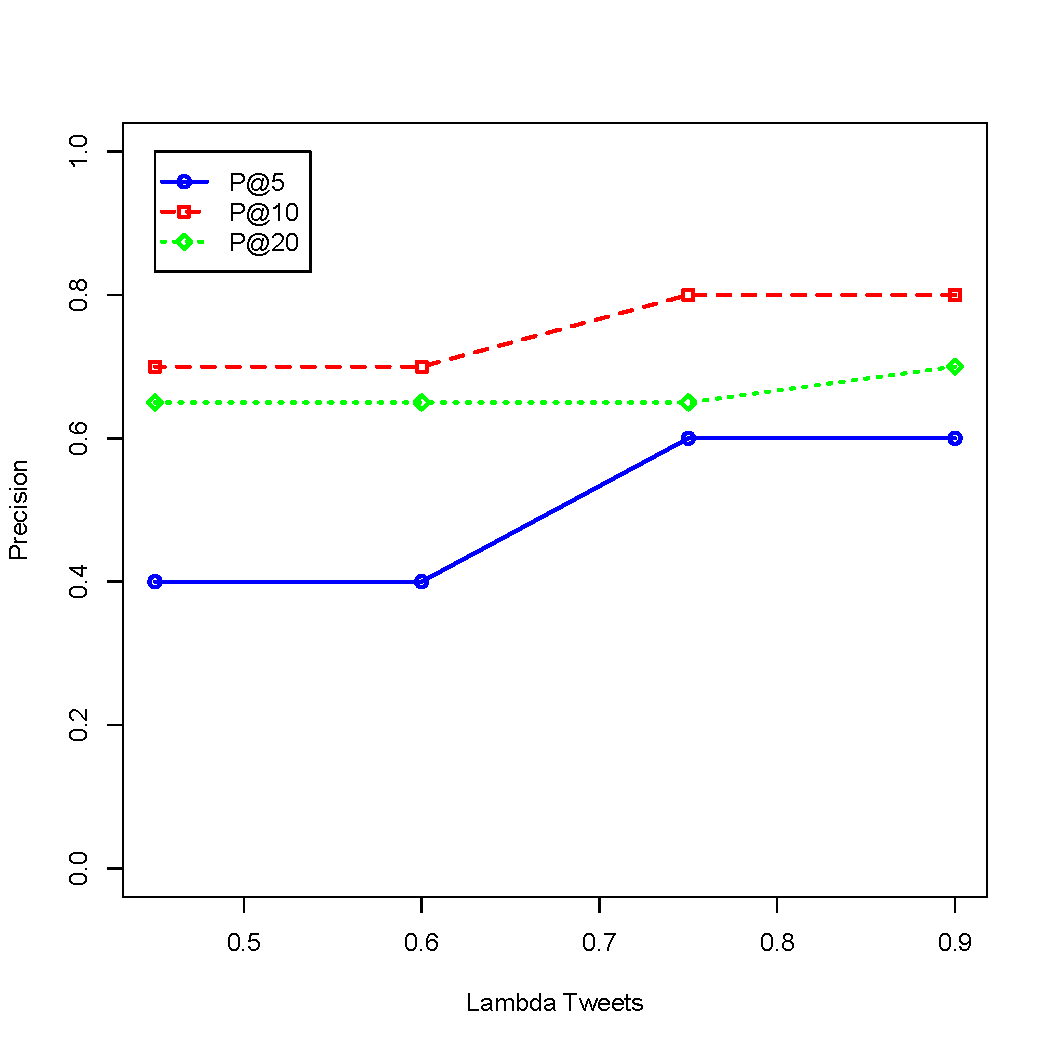
\includegraphics[scale=0.75]{Ki_Varying_LambdaTweets_UserResults}
  \caption[User recommendation results for user $K_{i}$ when varying $\lambda_{tweets}$]{User recommendation results for user $K_{i}$ when varying $\lambda_{tweets}$. The value of $\lambda_{users}$ is held constant at 0.7.}
  \label{fig:UsersForVaryingLambdaTweets}
\end{figure}
\begin{figure}
  \centering
  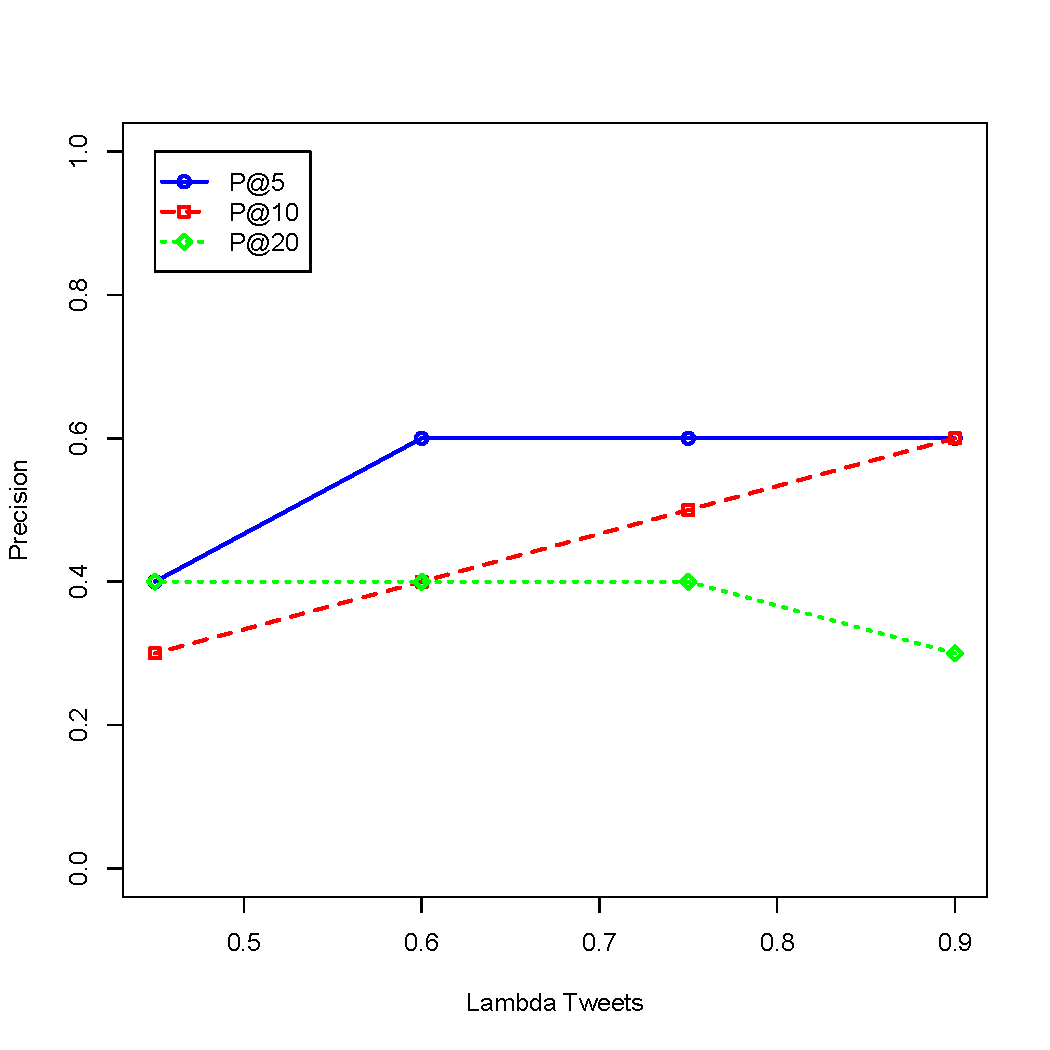
\includegraphics[scale=0.75]{Ki_Varying_LambdaTweets_TweetResults}
  \caption[Tweet recommendation results for user $K_{i}$ when varying $\lambda_{tweets}$]{Tweet recommendation results for user $K_{i}$ when varying $\lambda_{tweets}$. The value of $\lambda_{users}$ is held constant at 0.7.}
  \label{fig:TweetsForVaryingLambdaTweets}
\end{figure}


Figure~\ref{fig:UsersForVaryingLambdaUsers} shows the results of the user recommendations for user $K_{i}$ when varying the $\lambda_{users}$ parameter, while Figure~\ref{fig:TweetsForVaryingLambdaUsers} shows the results of the tweet recommendations for user $K_{i}$ when varying the $\lambda_{users}$ parameter. Both of these graphs confirm that a value of lambda tweets too close to 1 will provide terrible results. Because the initial scores for the users are so good, it does not particularly matter how close to 0 the value of lambda users gets.

\begin{figure}
  \centering
  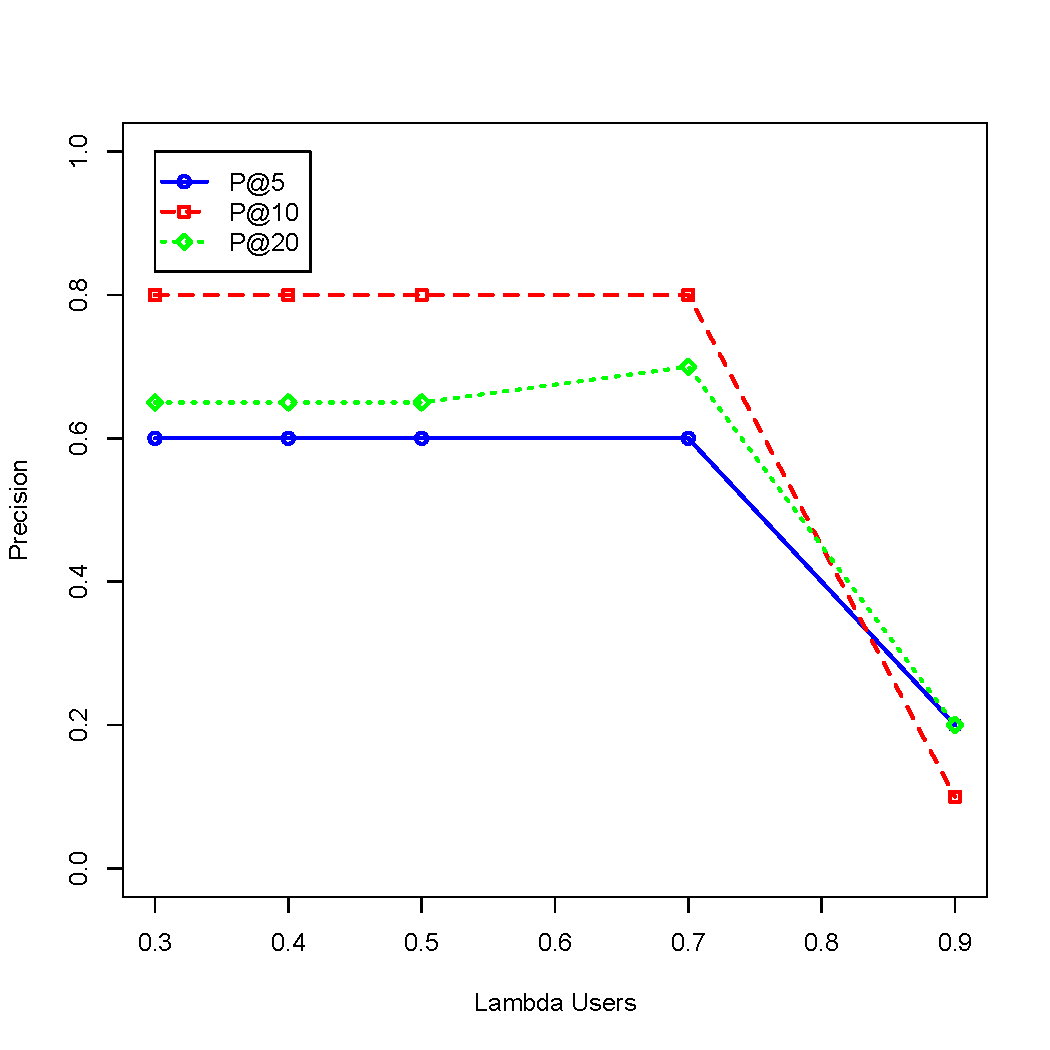
\includegraphics[scale=0.75]{Ki_Varying_LambdaUsers_UserResults}
  \caption[User recommendation results for user $K_{i}$ when varying $\lambda_{users}$]{User recommendation results for user $K_{i}$ when varying $\lambda_{users}$. The value of $\lambda_{tweets}$ is held constant at 0.9.}
  \label{fig:UsersForVaryingLambdaUsers}
\end{figure}
\begin{figure}
  \centering
  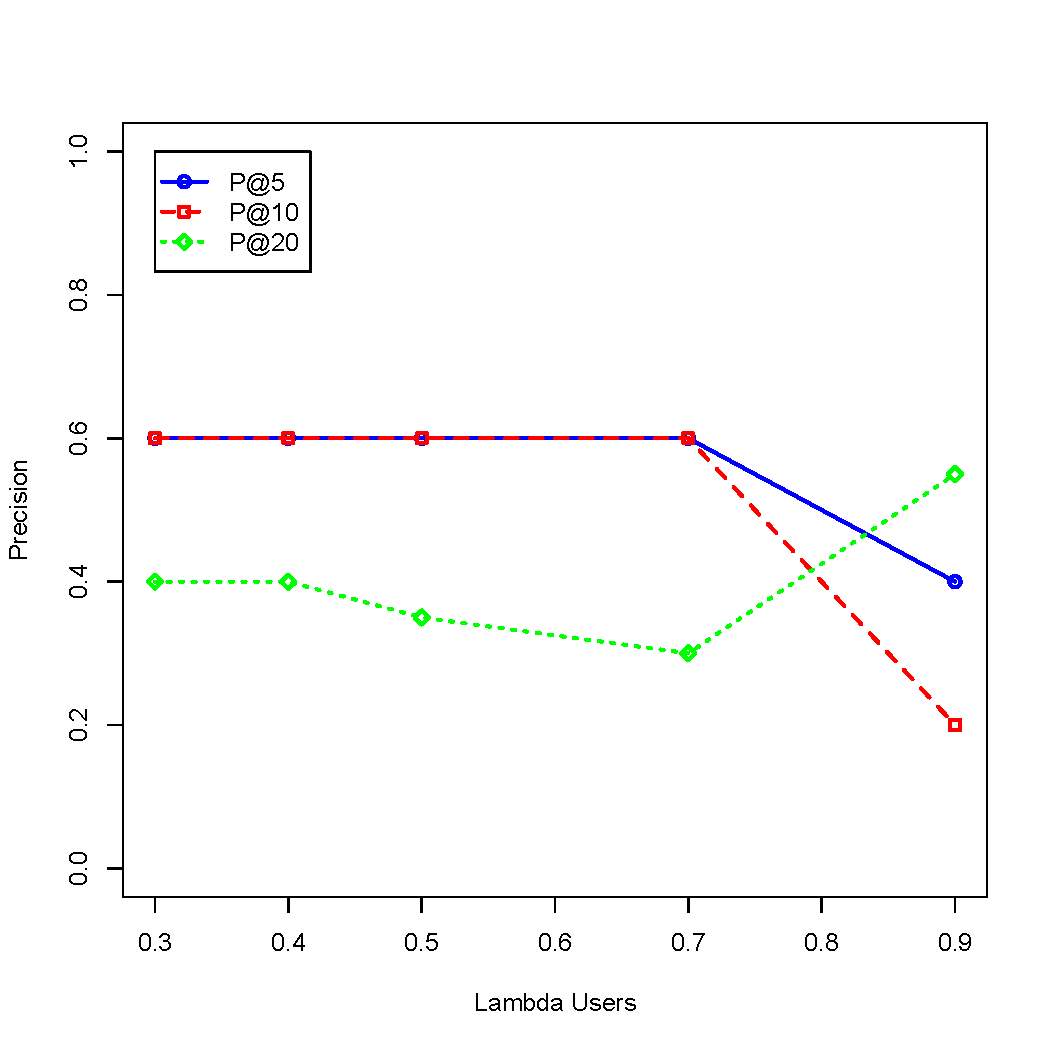
\includegraphics[scale=0.75]{Ki_Varying_LambdaUsers_TweetResults}
  \caption[Tweet recommendation results for user $K_{i}$ when varying $\lambda_{users}$]{Tweet recommendation results for user $K_{i}$ when varying $\lambda_{users}$. The value of $\lambda_{tweets}$ is held constant at 0.9.}
  \label{fig:TweetsForVaryingLambdaUsers}
\end{figure}


Another test was undertaken for user $K_{j}$, which was to hold $\lambda_{users}$ constant at 0.9 while varying the tweets parameter. Though not many data points were collected, it does still suggest that keeping the value of the $\lambda_{tweets}$ parameter closer to 1 is preferable. The graph for the user recommendation results on this data is shown in Figure~\ref{fig:KjUsersForVaryingLambdaTweets}, while the graph for the user recommendation results on this data is shown in Figure~\ref{fig:KjTweetsForVaryingLambdaTweets}. The results are not as good as when the value of $\lambda_{users}$ is closer to the optimal values revealed in the other experiments in this section.

\begin{figure}
  \centering
  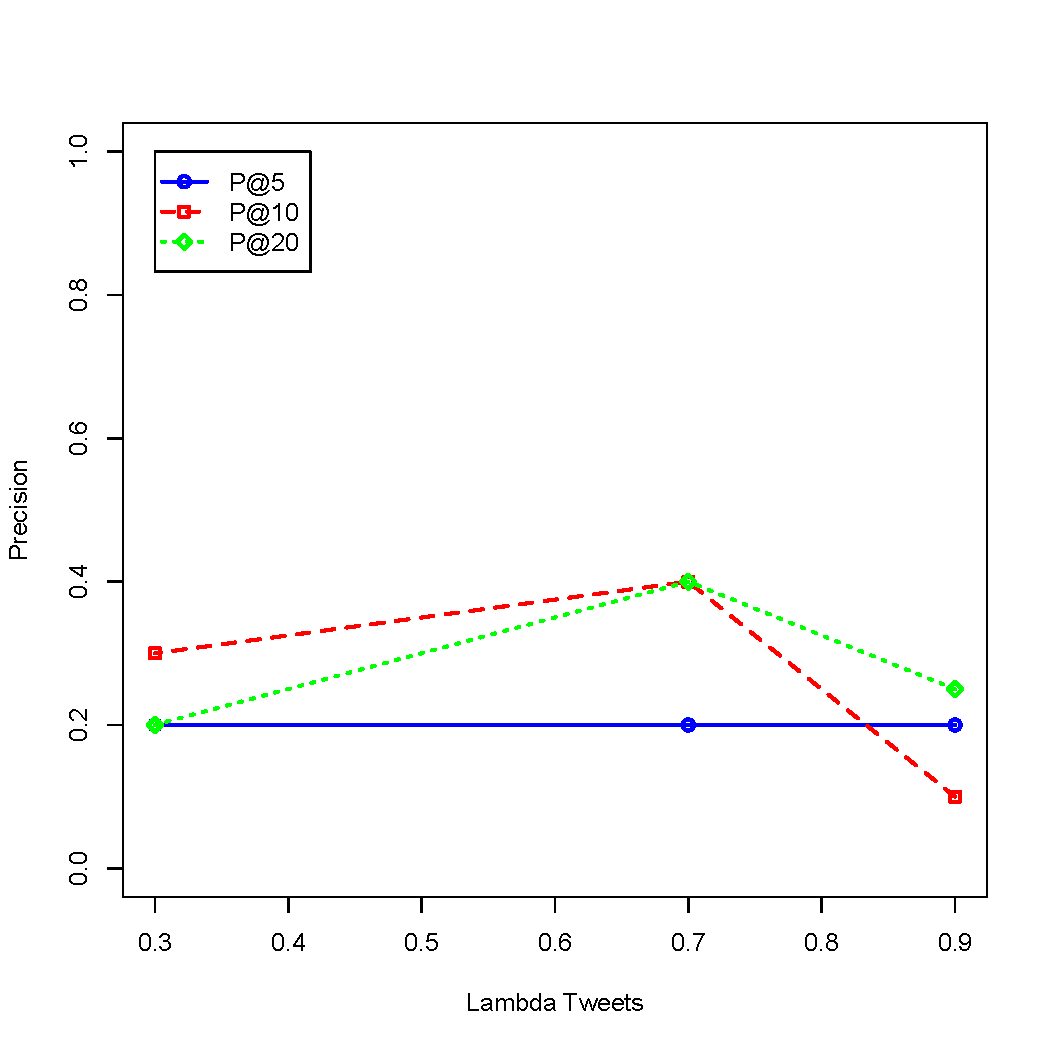
\includegraphics[scale=0.75]{Kj_Varying_LambdaTweets_UserResults}
  \caption[User recommendation results for user $K_{j}$ when varying $\lambda_{tweets}$]{User recommendation results for user $K_{j}$ when varying $\lambda_{tweets}$. The value of $\lambda_{users}$ is held constant at 0.9.}
  \label{fig:KjUsersForVaryingLambdaTweets}
\end{figure}
\begin{figure}
  \centering
  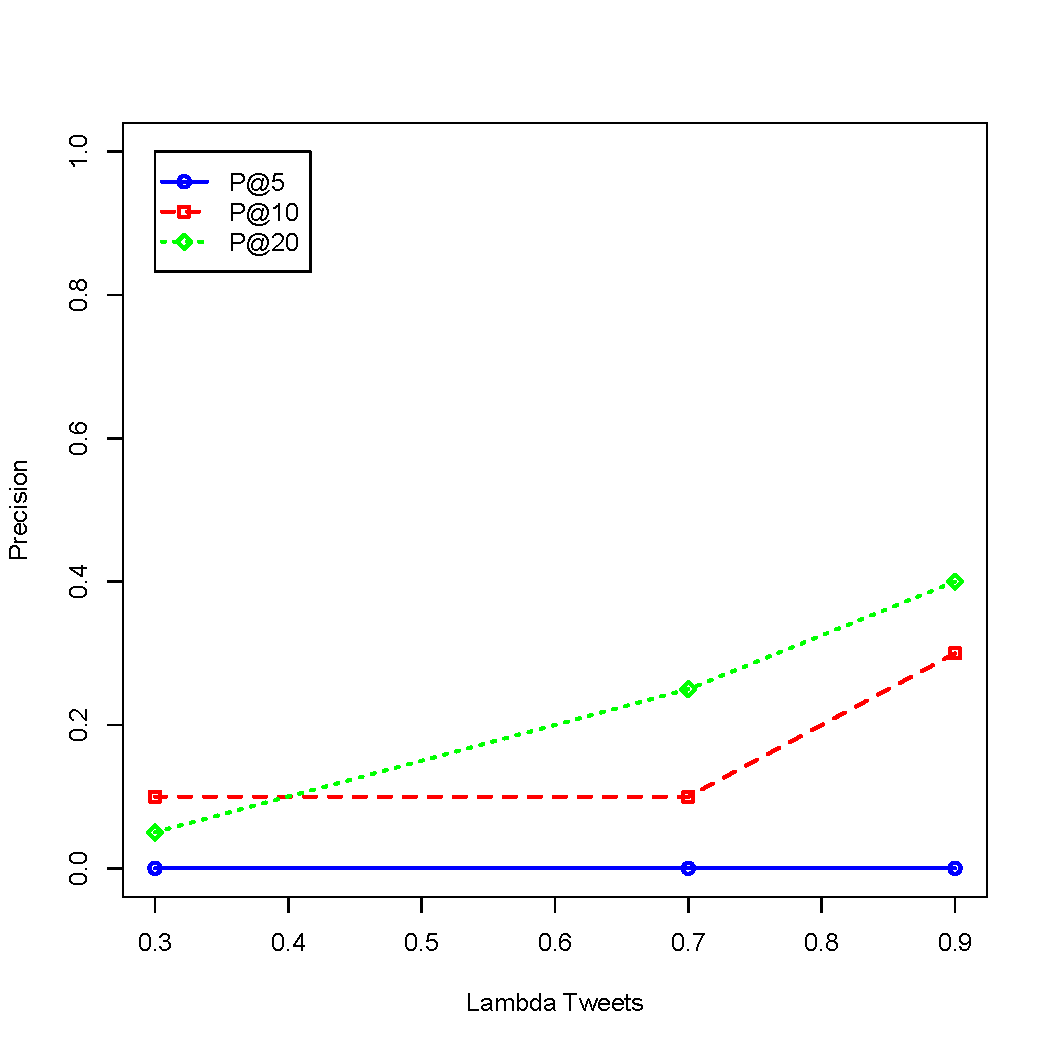
\includegraphics[scale=0.75]{Kj_Varying_LambdaTweets_TweetResults}
  \caption[Tweet recommendation results for user $K_{j}$ when varying $\lambda_{tweets}$]{Tweet recommendation results for user $K_{j}$ when varying $\lambda_{tweets}$. The value of $\lambda_{users}$ is held constant at 0.9.}
  \label{fig:KjTweetsForVaryingLambdaTweets}
\end{figure}

A final experiment on the lambda parameters was undertaken which moved both $\lambda$ parameters to 1, thereby removing much of the impact of the initial scores. The results for this configuration were terrible, with the precision for both tweets and users being 0.2, the average scores being between 2.5 and 2.75, and no scores of 5 for any of the user recommendations. The results for this experiment are included as part of the experiments on varying the types of edge included in the algorithm described in Section~\ref{sec:VaryingEdgeTypes}.



\subsection{Varying Edge Types Included}
\label{sec:VaryingEdgeTypes}

As was mentioned in Chapter 4, the algorithm was slow to run due to database access times. This made it difficult to experiment with removing edge types because with twelve different edge types there were a large number of possible combinations that could have been removed. Instead, the experiments focused on removing the edge types that seemed like they might be less valuable.

Recall the edge types from Table~\ref{tab:EdgeTypes}. The retweet, mention, and at-reply edges connect the user who was retweeted, mentioned, or at-replied to with the tweet that retweeted, mentioned, or at-replied to them. The logic behind this was previously discussed, but the link is a tenuous one and thus these are prime candidates for removal to see the effect on the results. Note that the other five retweet, mention, and at-reply edges remained in place.

There were 292,475 edges of these types, which is a very small amount in the context of 120 million total edges, and as can be seen from the results from removing these edges shown in Table~\ref{tab:Remove369}, removing these edges had very little impact on the overall quality of the results when compared with the baseline results already presented, and what little impact there was tended to be negative. This experiment was done for user $K_{i}$ only and it is difficult to draw too many conclusions from such a small smaple size, but since the edges do not seem to be particularly valuable they could perhaps be removed from the graph entirely in order to speed up the algorithm.


\begin{table}
\centering
\begin{tabular}{l|p{2cm}|p{2cm}|p{2cm}|p{2cm}}
{\bf Metric} & {\bf $K_{i}$ Base Config. User Scores} & {\bf $K_{j}$ User Scores} & {\bf $K_{i}$ Base Config. Tweet Scores} & {\bf $K_{j}$ Tweet Scores} \\ \hline
P@5   & 0.6 & 0.6 & 0.6 & 0.4 \\ \hline
P@10 & 0.8 & 0.8 & 0.6 & 0.5 \\ \hline
P@15 & 0.733 & 0.666 & 0.4 & 0.333 \\ \hline
P@20 & 0.7 & 0.65 & 0.3 & 0.25 \\ \hline

Avg. Score @5   & 3.0 & 3.0 & 3.4 & 3.4 \\ \hline
Avg. Score @10 & 3.7 & 3.7 & 3.3 & 3.4 \\ \hline
Avg. Score @15 & 3.733 & 3.6 & 2.933 & 2.866 \\ \hline
Avg. Score @20 & 3.65 & 3.6 & 2.9 & 2.7 \\ \hline

\% 5s@5    & 20\% & 20\% & - & - \\ \hline
\% 5s@10  & 30\% & 30\% & - & - \\ \hline
\% 5s@15  & 26.6\% & 26.6\% & - & - \\ \hline
\% 5s@20  & 20\% & 20\% & - & - \\

\end{tabular}
\caption[Results of removing the simple retweet, mention, and @reply edges.]{The tweet score and user score results for user $K_{i}$ when removing the simple retweet, mention, and @reply edges.}
\label{tab:Remove369}
\end{table}



The results from removing one or both of the types of content edges were only slightly clearer, though the impact improved the results rather than hurting them. Two basic experiments were run: one that removed all content edges (cf Table~\ref{tab:RemoveContent}) and one that removed only the hashtag edges (cf Table~\ref{tab:RemoveHashtags}). There were a lot of the content edges: about 42 million hashtag edges and about 38 million entity-based edges. It was surprising, then, when removing them had such a small effect. Comparing the results in Table~\ref{tab:RemoveContent} with the baseline results already presented shows very little difference. As with the other experiment with removing edges, this experiment was only run for user $K_{i}$.

\begin{table}
\centering
\begin{tabular}{l|p{2.2cm}|p{2.2cm}|p{2.2cm}|p{2.2cm}}
{\bf Metric} & {\bf $K_{i}$ Base User Scores} & {\bf $K_{i}$ User Scores} & {\bf $K_{i}$ Base Tweet Scores} & {\bf $K_{i}$ Tweet Scores} \\ \hline
P@5   & 0.6 & 0.6 & 0.6 & 0.6 \\ \hline
P@10 & 0.8 & 0.8 & 0.6 & 0.6 \\ \hline
P@15 & 0.733 & 0.866 & 0.4 & 0.466 \\ \hline
P@20 & 0.7 & 0.8 & 0.3 & 0.45 \\ \hline

Avg. Score @5   & 3.0 & 2.8 & 3.4 & 3.6 \\ \hline
Avg. Score @10 & 3.7 & 3.5 & 3.3 & 3.7 \\ \hline
Avg. Score @15 & 3.733 & 3.8 & 2.933 & 3.333 \\ \hline
Avg. Score @20 & 3.65 & 3.7 & 2.9 & 3.25 \\ \hline

\% 5s@5    & 20\% & 0\% & - & - \\ \hline
\% 5s@10  & 30\% & 10\% & - & - \\ \hline
\% 5s@15  & 26.6\% & 20\% & - & - \\ \hline
\% 5s@20  & 20\% & 20\% & - & - \\

\end{tabular}
\caption[Results of removing all content edges]{Results for user $K_{i}$ from removing all content edges, as compared with the base configuration}
\label{tab:RemoveContent}
\end{table}


\begin{table}
\centering
\begin{tabular}{l|p{2.2cm}|p{2.2cm}|p{2.2cm}|p{2.2cm}}
{\bf Metric} & {\bf $K_{i}$ Base User Scores} & {\bf $K_{i}$ User Scores} & {\bf $K_{i}$ Base Tweet Scores} & {\bf $K_{i}$ Tweet Scores} \\ \hline
P@5   & 0.6 & 0.6 & 0.6 & 0.6 \\ \hline
P@10 & 0.8 & 0.8 & 0.6 & 0.7 \\ \hline
P@15 & 0.733 & 0.733 & 0.4 & 0.533 \\ \hline
P@20 & 0.7 & 0.7 & 0.3 & 0.45 \\ \hline

Avg. Score @5   & 3.0 & 3.0 & 3.4 & 3.4 \\ \hline
Avg. Score @10 & 3.7 & 3.7 & 3.3 & 3.7 \\ \hline
Avg. Score @15 & 3.733 & 3.666 & 2.933 & 3.4 \\ \hline
Avg. Score @20 & 3.65 & 3.65 & 2.9 & 3.25 \\ \hline

\% 5s@5    & 20\% & 20\% & - & - \\ \hline
\% 5s@10  & 30\% & 30\% & - & - \\ \hline
\% 5s@15  & 26.6\% & 26.6\% & - & - \\ \hline
\% 5s@20  & 20\% & 20\% & - & - \\

\end{tabular}
\caption[Results of removing hashtag edges only]{Results for user $K_{i}$ from removing the hashtags edges only, as compared with the base configuration}
\label{tab:RemoveHashtags}
\end{table}


In order to attempt to isolate the effect of removing the edges from the effect of the initial scores, the removal of the content edges was also performed with both $\lambda$ parameters set to 1. The results for this are particularly interesting in that the results for the quality of the user recommendations were much lower than the default configuration and even lower than with the content edges in place, while the tweet scores improved greatly. This result is shown in Table~\ref{tab:RemoveContentLambdasAt1}, which compares the results of the user and tweet recommendations for user $K_{i}$ with the content edges in place but the $\lambda$ parameters set to 1 and the recommendations with the $\lambda$ parameters set to 1 but the content edges removed. As with all of the experimental variations described here, the sample size is too small to draw any firm conclusions, but it still suggests an interesting avenue for further exploration in the future.


\begin{table}
\centering
\begin{tabular}{l|p{2cm}|p{2cm}|p{2cm}|p{2cm}}
{\bf Metric} & {\bf $\lambda_{t,u}=1$ Base User Scores} & {\bf User Scores} & {\bf $\lambda_{t,u}=1$ Base Tweet Scores} & {\bf Tweet Scores} \\ \hline
P@5   & 0.0 & 0.2 & 0.2 & 0.6 \\ \hline
P@10 & 0.2 & 0.1 & 0.2 & 0.7 \\ \hline
P@15 & 0.2 & 0.133 & 0.2 & 0.533 \\ \hline
P@20 & 0.2 & 0.1 & 0.2 & 0.45 \\ \hline

Avg. Score @5   & 2.4 & 2.4 & 2.8 & 3.8 \\ \hline
Avg. Score @10 & 2.7 & 2.3 & 2.8 & 3.9 \\ \hline
Avg. Score @15 & 2.8 & 2.2 & 2.733 & 3.4 \\ \hline
Avg. Score @20 & 2.6 & 2.05 & 2.7 & 3.15 \\ \hline

\% 5s@5    & 0\% & 0\% & - & - \\ \hline
\% 5s@10  & 0\% & 0\% & - & - \\ \hline
\% 5s@15  & 0\% & 0\% & - & - \\ \hline
\% 5s@20  & 0\% & 0\% & - & - \\

\end{tabular}
\caption[Results of removing content edges and setting $\lambda$ parameters to 1]{The tweet score and user score results for user $K_{i}$ when removing the content edges with the $\lambda$ parameters set to 1}
\label{tab:RemoveContentLambdasAt1}
\end{table}

One final test on removing edges combined the two main edge types that were experimented on by removing the retweet, mention, and at-reply edges in addition to the two types of content edges. Again, the $\lambda$ parameters were set to 1 in an attempt to remove the impact of the initial scores on the outcome. For the user recommendations these results were slightly better than those from removing only the content edges, while for the tweet recommendations they were more mixed, with the top 10 showing worse results and the rest of the top 20 showing improved results. The usual caveats about small sample size apply here as well, of course.

\begin{table}
\centering
\begin{tabular}{l|p{2cm}|p{2cm}|p{2cm}|p{2cm}}
{\bf Metric} & {\bf $\lambda_{t,u}=1$ Base User Scores} & {\bf User Scores} & {\bf $\lambda_{t,u}=1$ Base Tweet Scores} & {\bf Tweet Scores} \\ \hline
P@5   & 0.0 & 0.4 & 0.2 & 0.6 \\ \hline
P@10 & 0.2 & 0.2 & 0.2 & 0.5 \\ \hline
P@15 & 0.2 & 0.2 & 0.2 & 0.666 \\ \hline
P@20 & 0.2 & 0.15 & 0.2 & 0.75 \\ \hline

Avg. Score @5   & 2.4 & 3.2 & 2.8 & 3.8 \\ \hline
Avg. Score @10 & 2.7 & 2.7 & 2.8 & 3.5 \\ \hline
Avg. Score @15 & 2.8 & 2.666 & 2.733 & 3.666 \\ \hline
Avg. Score @20 & 2.6 & 2.15 & 2.7 & 3.75 \\ \hline

\% 5s@5    & 0\% & 0\% & - & - \\ \hline
\% 5s@10  & 0\% & 0\% & - & - \\ \hline
\% 5s@15  & 0\% & 0\% & - & - \\ \hline
\% 5s@20  & 0\% & 0\% & - & - \\

\end{tabular}
\caption[Results from removing content edges and retweet, mention, and @reply edges]{The tweet score and user score results for user $K_{i}$ when removing the content edges and the simple retweet, mention, and @reply edges with the $\lambda$ parameters set to 1.}
\label{tab:RemoveContentAnd369LambdasAt1}
\end{table}


\subsection{Varying Edge Weights}

The slowness of running the algorithm made experimentation on edge weights particularly difficult because with so many different edges and possible weightings for them a rigorous experiment would require far more time than was available. As such, the experiments which were done were based largely on intuition and were small in number, with only four different weightings being explored.

The experiments done here were performed on user $K_{j}$, with directionality per the default, though authorship edges were bi-directional. Table~\ref{tab:EdgeWeightsUsed} shows the weights that were used for each edge type in each experiment. Table~\ref{tab:WeightsTestsUsers} shows the results for each experiment on the user recommendations and Table~\ref{tab:WeightsTestsTweets} shows the results for each experiment on the tweet recommendations. Note that the edges corresponding to basic retweets, mentions, and at replies were not included for any of these experiments, and thus no weights are listed for these edge types.

The methodology used was to sum the total weight of all edges emanating from a vertex, and the chance of taking a particular edge was just the weight of that edge's type divided by the total weight of all edges. So if a particular vertex had two edges with a weight of 2 each and one edge with a weight of  0.5 then the total weight would be 4.5, so the chance of going to each of the edges with weight 2 would be $2 \div 4.5 = 0.44$ and the chance of going to the edge with weight 0.5 would be $0.5 \div 4.5 = 0.11$.


\begin{table}
\centering
\begin{tabular}{l|p{1.5cm}|p{1.5cm}|p{1.5cm}|p{1.5cm}}
{\bf Edge Type} & {\bf Test 1 Weight} & {\bf Test 2 Weight} & {\bf Test 3 Weight} & {\bf Test 4 Weight} \\ \hline
Authorship & 2 & 2 & 2 & 4 \\ \hline
Follower & 1.25 & 1.25 & 1.25 & 1.5 \\ \hline
Retweet Followees & 2 & 3 & 3 & 3 \\ \hline
Retweet Followers & 0.75 & 1.25 & 1.25 & 1.25 \\ \hline
Mention Followees & 2 & 2 & 2 & 1.5 \\ \hline
Mention Followers & 0.75 & 1 & 1 & 1 \\ \hline
@reply Content & 0.5 & 0.5 & 0.25 & 0.5 \\ \hline
Hashtag & 1 & 1 & 3.5 & 1 \\ \hline
Content & 1 & 1 & 1.5 & 1 \\
\end{tabular}
\caption{Edge weights used for each experiment }
\label{tab:EdgeWeightsUsed}
\end{table}

\begin{table}
\centering
\begin{tabular}{l|p{1.5cm}|p{1.5cm}|p{1.5cm}|p{1.5cm}|p{1.5cm}}
{\bf Metric} & {\bf $K_{j}$ Base User Scores} & {\bf Test 1 User Scores} & {\bf Test 2 User Scores} & {\bf Test 3 User Scores} & {\bf Test 4 User Scores} \\ \hline
P@5   & 0.6 & 0.6 & 0.6 & 0.6 & 0.6 \\ \hline
P@10 & 0.6 & 0.6 & 0.6 & 0.6 & 0.6 \\ \hline
P@15 & 0.6 & 0.533 & 0.6 & 0.6 & 0.6 \\ \hline
P@20 & 0.55 & 0.6 & 0.65 & 0.6 & 0.6 \\ \hline

Avg. Score @5   & 3.4 & 3.4 & 3.4 & 3.4 & 3.4 \\ \hline
Avg. Score @10 & 3.5 & 3.7 & 3.7 & 3.7 & 3.7 \\ \hline
Avg. Score @15 & 3.6 & 3.4 & 3.666 & 3.666 & 3.666 \\ \hline
Avg. Score @20 & 3.35 & 3.5 & 3.65 & 3.65 & 3.65 \\ \hline

\% 5s@5    & 20\% & 40\% & 40\% & 40\% & 40\% \\ \hline
\% 5s@10  & 40\% & 40\% & 40\% & 40\% & 40\% \\ \hline
\% 5s@15  & 33.3\% & 33.3\% & 40\% & 40\% & 40\% \\ \hline
\% 5s@20  & 25\% & 30\% & 30\% & 30\% & 30\% \\
\end{tabular}
\caption[User recommendation results when varying the edge weights]{Results of the user recommendations for user $K_{j}$ when varying the weights of the edges}
\label{tab:WeightsTestsUsers}
\end{table}


\begin{table}
\centering
\begin{tabular}{l|p{1.5cm}|p{1.5cm}|p{1.5cm}|p{1.5cm}|p{1.5cm}}
{\bf Metric} & {\bf $K_{j}$ Base Tweet Scores} & {\bf Test 1 Tweet Scores} & {\bf Test 2 Tweet Scores} & {\bf Test 3 Tweet Scores} & {\bf Test 4 Tweet Scores} \\ \hline
P@5   & 0.0 & 0.4 & 0.4 & 0.4 & 0.4 \\ \hline
P@10 & 0.2 & 0.3 & 0.4 & 0.4 & 0.4 \\ \hline
P@15 & 0.4 & 0.4 & 0.4 & 0.4 & 0.4 \\ \hline
P@20 & 0.4 & 0.35 & 0.35 & 0.35 & 0.35 \\ \hline

Avg. Score @5   & 2.8 & 3.4 & 3.4 & 3.4 & 3.4 \\ \hline
Avg. Score @10 & 3.1 & 3.3 & 3.4 & 3.4 & 3.4 \\ \hline
Avg. Score @15 & 3.266 & 3.4 & 3.4 & 3.4 & 3.4 \\ \hline
Avg. Score @20 & 3.3 & 3.3 & 3.3 & 3.3 & 3.4 \\
\end{tabular}
\caption[Tweet recommendation results when varying the edge weights]{Results of the tweet recommendations for user $K_{j}$ when varying the weights of the edges}
\label{tab:WeightsTestsTweets}
\end{table}

One very clear result from the experiments is that none of them gave results which were particularly distinct, though the results from the fourth experiment were perhaps slightly better. The most likely reason for this is that the values for the weights of the various edges were not very distinct between the different experiments. Instead, they were based on a few assumptions, such as the fact that retweets, followers, and authorship edges are all very important. Existing research and some of the other experiments support these intuitions, but the experiments run here neither proved nor disproved them.


\subsection{Varying Edge Directionality}
\label{sec:VaryingEdgeDirectionality}

The directionality of the edges when producing the baseline results described in Section~\ref{sec:BaselineResults} followed the description in Table~\ref{tab:EdgeTypes}. As shown in that section, this directionality produced generally good recommendations for both users and tweets.

One obvious variation on these baseline results is to remove edge directionality altogether and assume that each edge type has an influence in both directions. For at least some of the edge types, this makes perfect sense. Consider the authorship edge, for example. It certainly makes sense that if a particular tweet received a high score because of something it was connected to then that score should be passed along to the author of the tweet. Similarly, a highly scoring user should obviously transfer some of that high score along to the tweets that they author.

Running the algorithm with all edge types being bi-directional was one of the first experiments that was run for user $U$. The results from doing this were very clearly terrible. The tweets were dominated by one or two users and the tweets of those users were political in nature and diametrically opposed to the political views of the distinguished user. On the scale used for the user study, all of these would have ranked as a 2 had user $U$ been part of the user study.

The reason for this was that the user who produced the tweets followed over 40,000 people, and today follows more than 80,000 people. Clearly this user does not interact with or even read all of the tweets from these 40,000 people, but the algorithm cannot take that into account. So because this user tweeted frequently and followed so many people, their tweets were highly scored by the system with bi-directional edges because each of their 19 tweets was connected to thousands of users whose scores all contributed to high scores for these tweets.

This result demonstrates that for the edges based on the network state it does not makes sense to vary the directionality of the edges, either by reversing them or by making them bi-directional. Take follower edges for example: clearly there is not an influence by a user on the tweets of someone they follow. This was the biggest issue in the experiment done with no directionality at all---it assumed influence where there was none and came up with correspondingly terrible results.

Eliminating the network edges from consideration then leaves only the two content-based edges and the authorship edge as candidates for changing directionality. With these edges it is not clear that any one direction should be the one that has the influence; for instance, it could make sense that all tweets on a given subject should provide their scores to a user or that a highly scoring user should provide an impact on all tweets mentioning subjects of a similar subject. Similarly, leaving these as bi-directional as in the default configuration also makes sense.


\begin{table}
\centering
\begin{tabular}{l|p{2.2cm}|p{2.2cm}|p{2.2cm}|p{2.2cm}}
{\bf Metric} & {\bf $K_{i}$ Base User Scores} & {\bf $K_{i}$ User Scores} & {\bf $K_{i}$ Base Tweet Scores} & {\bf $K_{i}$ Tweet Scores} \\ \hline
P@5   & 0.6 & 0.6 & 0.6 & 0.6 \\ \hline
P@10 & 0.8 & 0.8 & 0.6 & 0.7 \\ \hline
P@15 & 0.733 & 0.866 & 0.4 & 0.533 \\ \hline
P@20 & 0.7 & 0.75 & 0.3 & 0.45 \\ \hline

Avg. Score @5   & 3.0 & 3.0 & 3.4 & 3.6 \\ \hline
Avg. Score @10 & 3.7 & 3.6 & 3.3 & 3.8 \\ \hline
Avg. Score @15 & 3.733 & 3.866 & 2.933 & 3.4 \\ \hline
Avg. Score @20 & 3.65 & 3.7 & 2.9 & 3.25 \\ \hline

\% 5s@5    & 20\% & 20\% & - & - \\ \hline
\% 5s@10  & 30\% & 20\% & - & - \\ \hline
\% 5s@15  & 26.6\% & 26.6\% & - & - \\ \hline
\% 5s@20  & 20\% & 20\% & - & - \\

\end{tabular}
\caption{Results for user $K_{i}$ when content edges are directed from tweet to user}
\label{tab:ContentTweetToUser}
\end{table}


\begin{table}
\centering
\begin{tabular}{l|p{2.2cm}|p{2.2cm}|p{2.2cm}|p{2.2cm}}
{\bf Metric} & {\bf $K_{i}$ Base User Scores} & {\bf $K_{i}$ User Scores} & {\bf $K_{i}$ Base Tweet Scores} & {\bf $K_{i}$ Tweet Scores} \\ \hline
P@5   & 0.6 & 0.6 & 0.6 & 0.8 \\ \hline
P@10 & 0.8 & 0.6 & 0.6 & 0.6 \\ \hline
P@15 & 0.733 & 0.733 & 0.4 & 0.466 \\ \hline
P@20 & 0.7 & 0.7 & 0.3 & 0.35 \\ \hline

Avg. Score @5   & 3.0 & 3.0 & 3.4 & 4.4 \\ \hline
Avg. Score @10 & 3.7 & 3.2 & 3.3 & 3.6 \\ \hline
Avg. Score @15 & 3.733 & 3.6 & 2.933 & 3.266 \\ \hline
Avg. Score @20 & 3.65 & 3.6 & 2.9 & 2.9 \\ \hline

\% 5s@5    & 20\% & 20\% & - & - \\ \hline
\% 5s@10  & 30\% & 10\% & - & - \\ \hline
\% 5s@15  & 26.6\% & 20\% & - & - \\ \hline
\% 5s@20  & 20\% & 20\% & - & - \\
\end{tabular}
\caption{Results for user $K_{i}$ when content edges are directed from user to tweet}
\label{tab:ContentUserToTweet}
\end{table}

Both directions for the content edges yield improved results for the tweet recommendations, which is quite a surprising result. Directing the content edges from tweet to user yields slightly better user recommendations, though the recommendations are quite good in both cases. Table~\ref{tab:ContentTweetToUser} shows the results when content edges are directed from tweet vertices to user vertices and Table~\ref{tab:ContentUserToTweet} shows the results when the content edges go in the other direction.


Experiments were also done with the authorship edge. By default this edge was directed from the user to the tweet, but as was previously discussed this could certainly have been bi-directional. The results shown in Table~\ref{tab:BiDirectionalAuthorKi} are from running the algorithm for user $K_{i}$ with all the standard edges and directions but with the authorship edge being bi-directional. Table~\ref{tab:BiDirectionalAuthorKj}, meanwhile, shows the same experiment for user $K_{j}$. The results for this configuration show that changing the direction of these 500,000 edges has almost no effect.

\begin{table}
\centering
\begin{tabular}{l|p{2.2cm}|p{2.2cm}|p{2.2cm}|p{2.2cm}}
{\bf Metric} & {\bf $K_{i}$ Base User Scores} & {\bf $K_{i}$ User Scores} & {\bf $K_{i}$ Base Tweet Scores} & {\bf $K_{i}$ Tweet Scores} \\ \hline
P@5   & 0.6 & 0.6 & 0.6 & 0.6 \\ \hline
P@10 & 0.8 & 0.8 & 0.6 & 0.5 \\ \hline
P@15 & 0.733 & 0.733 & 0.4 & 0.4 \\ \hline
P@20 & 0.7 & 0.65 & 0.3 & 0.4 \\ \hline

Avg. Score @5   & 3.0 & 3.0 & 3.4 & 3.6 \\ \hline
Avg. Score @10 & 3.7 & 3.7 & 3.3 & 3.3 \\ \hline
Avg. Score @15 & 3.733 & 3.733 & 2.933 & 3.0 \\ \hline
Avg. Score @20 & 3.65 & 3.6 & 2.9 & 3.1 \\ \hline

\% 5s@5    & 20\% & 20\% & - & - \\ \hline
\% 5s@10  & 30\% & 30\% & - & - \\ \hline
\% 5s@15  & 26.6\% & 26.6\% & - & - \\ \hline
\% 5s@20  & 20\% & 20\% & - & - \\
\end{tabular}
\caption{Results for user $K_{i}$ when the authorship edge is bi-directional.}
\label{tab:BiDirectionalAuthorKi}
\end{table}



\begin{table}
\centering
\begin{tabular}{l|p{2.2cm}|p{2.2cm}|p{2.2cm}|p{2.2cm}}
{\bf Metric} & {\bf $K_{j}$ Base User Scores} & {\bf $K_{j}$ User Scores} & {\bf $K_{j}$ Base Tweet Scores} & {\bf $K_{j}$ Tweet Scores} \\ \hline
P@5   & 0.6 & 0.6 & 0.0 & 0.0 \\ \hline
P@10 & 0.6 & 0.6 & 0.2 & 0.2 \\ \hline
P@15 & 0.6 & 0.6 & 0.4 & 0.266 \\ \hline
P@20 & 0.55 & 0.6 & 0.4 & 0.3 \\ \hline

Avg. Score @5   & 3.4 & 3.4 & 2.8 & 2.8 \\ \hline
Avg. Score @10 & 3.5 & 3.7 & 3.1 & 3.0 \\ \hline
Avg. Score @15 & 3.6 & 3.6 & 3.266 & 3.133 \\ \hline
Avg. Score @20 & 3.35 & 3.5 & 3.3 & 3.2 \\ \hline

\% 5s@5    & 20\% & 40\% & - & - \\ \hline
\% 5s@10  & 40\% & 40\% & - & - \\ \hline
\% 5s@15  & 33.3\% & 33\% & - & - \\ \hline
\% 5s@20  & 25\% & 30\% & - & - \\

\end{tabular}
\caption{Results for user $K_{j}$ when the authorship edge is bi-directional.}
\label{tab:BiDirectionalAuthorKj}
\end{table}



\subsection{Combined Configuration}
\label{sec:CombinedConfiguration}

Most of the experiments showed very mixed results for individual variations, with most of the experiments making very little difference on the final outcome. The values for the $\lambda$ parameters were fairly clear, but changing the included edges and the edge directions had little effect. Still, one thing that has not been explored thus far is a combination of some of these different features. The results in this section combine some of the past experiments into a combined configuration in hopes that the combination will produce better results than the generally middling results of the previous experiments. Unfortunately, the results are generally comparable to those of the baseline configuration, though perhaps a more robust experiment which studied more users would reveal more clear-cut results.

Table~\ref{tab:BiAuthorNo369Ki} shows the results for user $K_{i}$ with the authorship edge being bi-directional and the simple retweet, mention, and at-reply edges being removed. As with many of the other experimental variations the results differ only slightly from the baseline results, and only one or two tweets and users are different. Table~\ref{tab:BiAuthorNo369Kj} shows the results of the same experiment for $K_{j}$, which shows slightly better results. The tweet recommendations for user $K_{j}$ do show quite a bit of improvement early in the recommendations list, though this is due in no small part to the fact that the baseline tweet results for this user were poor to begin with.

By default, the algorithm ignores the duplicate edges of the same type linking a user and a tweet that exist in the graph. As an additional experiment on user $K_{i}$, the experiment just described was repeated with the duplicate edges in the graph being left in. The results for this were identical to the results when leaving these edges out. This surprising result suggests a possible way to speed up the algorithm, since more than 10 million of the edges are duplicates.


\begin{table}
\centering
\begin{tabular}{l|p{2.2cm}|p{2.2cm}|p{2.2cm}|p{2.2cm}}
{\bf Metric} & {\bf $K_{i}$ Base User Scores} & {\bf $K_{i}$ User Scores} & {\bf $K_{i}$ Base Tweet Scores} & {\bf $K_{i}$ Tweet Scores} \\ \hline
P@5   & 0.6 & 0.6 & 0.6 & 0.4 \\ \hline
P@10 & 0.8 & 0.8 & 0.6 & 0.4 \\ \hline
P@15 & 0.733 & 0.666 & 0.4 & 0.4 \\ \hline
P@20 & 0.7 & 0.6 & 0.3 & 0.3 \\ \hline

Avg. Score @5   & 3.0 & 3.0 & 3.4 & 3.4 \\ \hline
Avg. Score @10 & 3.7 & 3.7 & 3.3 & 3.2 \\ \hline
Avg. Score @15 & 3.733 & 3.6 & 2.933 & 3.066 \\ \hline
Avg. Score @20 & 3.65 & 3.55 & 2.9 & 2.8 \\ \hline

\% 5s@5    & 20\% & 20\% & - & - \\ \hline
\% 5s@10  & 30\% & 30\% & - & - \\ \hline
\% 5s@15  & 26.6\% & 26.6\% & - & - \\ \hline
\% 5s@20  & 20\% & 20\% & - & - \\
\end{tabular}
\caption[Results for user $K_{i}$ using combined configuration 1]{Results for user $K_{i}$ with the authorship edge being bi-directional and the retweet, mention, and @reply edges not included.}
\label{tab:BiAuthorNo369Ki}
\end{table}


\begin{table}
\centering
\begin{tabular}{l|p{2.2cm}|p{2.2cm}|p{2.2cm}|p{2.2cm}}
{\bf Metric} & {\bf $K_{j}$ Base User Scores} & {\bf $K_{j}$ User Scores} & {\bf $K_{j}$ Base Tweet Scores} & {\bf $K_{j}$ Tweet Scores} \\ \hline
P@5   & 0.6 & 0.6 & 0.0 & 0.4 \\ \hline
P@10 & 0.6 & 0.6 & 0.2 & 0.4 \\ \hline
P@15 & 0.6 & 0.6 & 0.4 & 0.333 \\ \hline
P@20 & 0.55 & 0.65 & 0.4 & 0.4 \\ \hline

Avg. Score @5   & 3.4 & 3.4 & 2.8 & 3.4 \\ \hline
Avg. Score @10 & 3.5 & 3.7 & 3.1 & 3.5 \\ \hline
Avg. Score @15 & 3.6 & 3.6 & 3.266 & 3.266 \\ \hline
Avg. Score @20 & 3.35 & 3.65 & 3.3 & 3.35 \\ \hline

\% 5s@5    & 20\% & 40\% & - & - \\ \hline
\% 5s@10  & 40\% & 40\% & - & - \\ \hline
\% 5s@15  & 33.3\% & 33.3\% & - & - \\ \hline
\% 5s@20  & 25\% & 30\% & - & - \\

\end{tabular}
\caption[Results for user $K_{j}$ using combined configuration 1]{Results for user $K_{j}$ with the authorship edge being bi-directional and the retweet, mention, and @reply edges not included.}
\label{tab:BiAuthorNo369Kj}
\end{table}

One final experiment was run on $K_{j}$, similar to those on user $K_{i}$, but with the two content edge types not included. The results for this experiment are shown in Table~\ref{tab:BiAuthorNo369NoContent} and show that the early tweet recommendations were much improved over the baseline, while the user recommendations were about the same.


\begin{table}
\centering
\begin{tabular}{l|p{2.2cm}|p{2.2cm}|p{2.2cm}|p{2.2cm}}
{\bf Metric} & {\bf $K_{j}$ Base User Scores} & {\bf $K_{j}$ User Scores} & {\bf $K_{j}$ Base Tweet Scores} & {\bf $K_{j}$ Tweet Scores} \\ \hline
P@5   & 0.6 & 0.6 & 0.0 & 0.6 \\ \hline
P@10 & 0.6 & 0.5 & 0.2 & 0.5 \\ \hline
P@15 & 0.6 & 0.533 & 0.4 & 0.466 \\ \hline
P@20 & 0.55 & 0.5 & 0.4 & 0.4 \\ \hline

Avg. Score @5   & 3.4 & 3.4 & 2.8 & 3.6 \\ \hline
Avg. Score @10 & 3.5 & 3.3 & 3.1 & 3.5 \\ \hline
Avg. Score @15 & 3.6 & 3.4 & 3.266 & 3.466 \\ \hline
Avg. Score @20 & 3.35 & 3.3 & 3.3 & 3.4 \\ \hline

\% 5s@5    & 20\% & 40\% & - & - \\ \hline
\% 5s@10  & 40\% & 30\% & - & - \\ \hline
\% 5s@15  & 33.3\% & 26.6\% & - & - \\ \hline
\% 5s@20  & 25\% & 25\% & - & - \\

\end{tabular}
\caption[Results for user $K_{j}$ using combined configuration 2]{Results for user $K_{j}$ with the authorship edge being bi-directional and the retweet, mention, @reply, hashtag, and entity-based edges not included.}
\label{tab:BiAuthorNo369NoContent}
\end{table}



\section{Dataset Biases}

The results described in this chapter revealed some issues that come with selecting tweets to use for such a study that can end up having a major impact on the final results.

One drawback of the Twitter network is that particular communities are often over-represented, which can make it more difficult to find relevant content for people not in those communities. The tweet recommendations here show that effect quite clearly. User $U$ is a part of the Silicon Valley entrepreneurship community, which is very strongly represented on Twitter. Within the 500,000 tweets studied here that user's results were very good since there were a large number of tweets that would be interesting to someone from that community. But the trade-off is that there were far fewer tweets of interest available for the other users who were not part of that community.

Another bias in the Twitter dataset is that the subjects of the tweets can be overwhelmed by one particular event. The day that the tweets used here were collected happened to be World AIDS Day in 2009, resulting in a much higher level of discussion of things related to that than would normally be expected. This also had the effect of limiting the number of interesting tweets for someone who wasn't interested in content related to World AIDS Day.

Finally, because of limitations within the Twitter API and limitations of storing and collecting a large amount of data, the Twitter data used here only represents 20-30\% of tweets during the time period. This results in a lot of cases where a retweet is among the recommendations while the original tweet was never seen. The results could be improved if the repeated retweets of the same tweet were removed from the recommendations in favour of the original tweet.

All of these biases were noticeable in the results, though the impact was generally not a major one and the algorithm still produced excellent recommendations. It would be interesting and valuable to study the effect that these biases have on the results, such as by studying a larger number of tweets, a more complete dataset, or multiple different time periods.

That is far from the only work that remains to be done in this still very new research area, of course. While the results here are very promising, the experiments and methodologies suggest that plenty of improvements could be made and further experiments performed to improve the results described in this chapter. The final chapter will discuss some of the other future work that could be done to expand on and improve this project as well as providing concluding remarks on the project as a whole.





